\documentclass[11pt,a4paper]{article}

%==============================================================================%

\usepackage{a4wide}
\usepackage{amsmath,amssymb}
\usepackage[utf8]{inputenc}
\usepackage{float}
\usepackage{graphicx}
\usepackage{listings}
\usepackage{multicol}

%==============================================================================%

\newcommand{\assignmentnumber}{2}
\newcommand{\modulus}[1]{\lvert#1\rvert}
\newcommand{\conjugate}[1]{\bar{#1}}
\newcommand{\degree}{^{\circ}}

\DeclareMathOperator{\re}{Re}
\DeclareMathOperator{\im}{Im}

\renewcommand\thesection{\assignmentnumber.\arabic{section}}
\renewcommand\thesubsection{\alph{subsection})}

%==============================================================================%

\title{MatIntro Pointopgave \assignmentnumber}
\author
{
    Casper B. Hansen\\
    University of Copenhagen\\
    {\tt fvx507@alumni.ku.dk}
}
\date{\today}

%==============================================================================%

\begin{document}

% \maketitle


% 2.1
\section
{
    \mdseries
    Regn TLO 3.4.12 uden brug af elektroniske hjælpemidler. Vis på en (gerne
    håndtegnet) skitse, hvordan løsningerne ligger i den komplekse plan.
    \\\indent
    Find de komplekse løsninger til ligningen $z^2 - 2iz - (1 + i) = 0$.
    Skriv svaret på formen $a + bi$.
}
Jvf. sætning 3.4.5[TL] har vi, at
\begin{align}
    z &= \frac{-b \pm \sqrt{b^2 - 4ac}}{2a} \\
      &= \frac{-(-2i)z \pm \sqrt{(-2i)^2 - 4 \cdot 1 \cdot (1 + i)}}{2 \cdot 1} \\
      &= iz \pm \frac{\sqrt{(-2i)^2 - (4 + 4i)}}{2} \\
      &= iz \pm \frac{1}{2} \sqrt{(-8 - 4i)}
\end{align}
Vi skal nu finde kvadratroden til $(-8 - 4i)$. Vi bestemme da først modulus;
\begin{align}
    \modulus{(-8 - 4i)} &= \sqrt{(-8)^2 + (-4)^2}
                         = \sqrt{64 + 16}
                         = \sqrt{80}
                         = \sqrt{2^4 \cdot 5}
                         = 4 \sqrt{5}
\end{align}
Til bestemmelse af argumentet har vi, at
\begin{align}
    \cos \theta = \frac{-8}{4 \sqrt{5}}
                = \frac{-2}{\sqrt{5}}
                = \frac{-2}{5} \sqrt{5}
    \quad
    \sin \theta = \frac{-4}{4 \sqrt{5}}
                = \frac{-1}{\sqrt{5}}
                = \frac{-1}{5} \sqrt{5}
\end{align}
Endvidere har vi da, at
\begin{align}
    \tan \theta = \frac{\sin \theta}{\cos \theta}
                = \frac{-1 / \sqrt{5}}{-2 / \sqrt{5}}
                = \frac{-1}{-2}
                = \frac{1}{2}
\end{align}
Vi har da, at
\begin{align}
    (-8 - 4i) &= 4 \sqrt{5} e^{\arctan(\frac{1}{2}) i}
\end{align}

% 2.2
\section
{
    \mdseries
    Betragt funktionen $f(x) = \frac{2x^2 - x - 1}{x^2 + 3x + 2}$, $x \in
    [0,\infty[$.
}
I det følgende vil jeg benævne $P(x) = 2x^2 - x - 1$ og
$Q(x) = x^2 + 3x + 2$, for $x \in [0,\infty[$.

\subsection{\mdseries Tegn funktionens graf med Maple.}
\begin{figure}[H]
    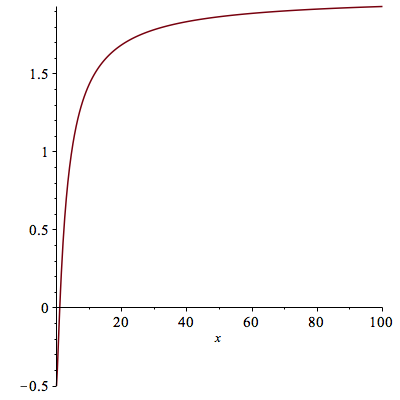
\includegraphics[scale=1.0]{figures/2-2a-fig-1.png}
\end{figure}

\subsection{\mdseries Udregn den afledede $f'(x)$ (benyt gerne Maple) og vis,
    at den positiv for alle $x \in [0,\infty[$.}

\begin{align}
    f'(x) &= \frac{P(x)' Q(x) - P(x) Q(x)'}{Q(x)^2} \\
          &= \frac{P(x)' Q(x)}{Q(x)} - \frac{P(x) Q(x)'}{Q(x)^2} \\
          &= \frac{4x - 1}{x^2 + 3x + 2} -
             \frac{(2x^2 - x - 1) (2x + 3)}{(x^2 + 3x + 2)^2}
\end{align}

\subsection{\mdseries Bestem $\lim_{n \rightarrow \infty}f(n)$ (benyt ikke
    Maple).}
Det fremgår tydeligt af grafen til $f$ at funktionen har asymptote i $y = 2$,
dette underbygges også af $f'$, da denne har asymptote i $y = 0$.

\subsection{\mdseries Bestem værdimængden for $f$.}
$V_f = [-0.5,2[$.

\subsection{\mdseries Lad $\epsilon = 0.1$. Bestem en værdi af $N$, som kan
    anvendes i TL definition 4.3.1, når denne definition benyttes på
    grænseovergangen i (c). Du må gerne benytte Maple til at finde en værdi
    af $N$, men du skal argumentere for, at den faktisk kan anvendes. Gentag
    for $\epsilon = 0.01$.}
...


% 2.3(iv)
\section
{
    \mdseries
    Denne opgave omhandler, hvor hurtigt kaniner kan formere sig under
    idealiserede forhold. Vi antager, at vi starter med par nyfødte kaniner,
    en han- og en hunkanin. Forestil dig, at kaniner kan formere sig, når de
    er 1 måned gamle, og en hunkanin har en drægtighedsperiode på 1 måned, så
    ved udgangen af den 2. måned kan hun-kaninen føde et nyt kaninpar (men det
    nye kuld kommer først til umiddelbart efter 2. måned, således at der i 2.
    måned stadig kun er 1 kaninpar.) Vi antager, at vores kaniner ikke dør,
    og der ved hver fødsel kommer et kaninpar bestående af en han- og en
    hunkanin.
    \\\indent
    Lad $n \in \mathbb{N}$ betegne måned nummer $n$, med $n=1$ som den
    første måned. Lad $F_n$ betegne antallet af kaninpar i måneden $n$. Hvis
    kaninerne får lov til at formere sig til frit, vil det samlede antal
    kaninpar være summen af par de to foregående måned.
}
\begin{align}
    F_{n+2} = F_n + F_{n+1}
\end{align}

\subsection
{
    \mdseries
    Giv en intuitiv forklaring på denne rekursionsformel. Hvad er
    begyndelsesbetingelserne $F_1$, $F_2$ i vores tilfælde? Bestem, hvor
    mange kaninpar der således vil være efter 1 år.
}
...

\subsection
{
    \mdseries
    Vis at elementerne i følgen ${F_n}$ opfylder $F_n \leq F_{n+1} \leq 2F_n$
    for ethvert $n \in \mathbb{N}$.
    \\\indent
    Vi definerer vækstraten for kaninbestanden ved $a_n =
    \frac{F_{n+1}}{F_n}$. Udregn vækstraten for $n = 1, 2, \dots, 12$ og
    illustrer de beregnede værdier af $a_n$ ved brug Maple.
}
...

\subsection
{
    \mdseries
    Anfør ud fra din illustration i (b) et træk ved den første del af følgen
    ${a_n}$, der taler for, at følgen konvergent. Vi tillader os nu at
    antage, at dette kan uddybes til et bevis for at følgen {\it er}
    konvergent.
    \\\indent
    Bestem grænseværdien, $a$, af $a_n$ for $n \rightarrow \infty$ uden brug
    af Maple. [Vink: opstil først rekursionsformlen $a_{n+1} = 1 +
    \frac{1}{a_n}$ ud fra (1) og se, hvad der sker når $n \rightarrow
    \infty$.]
}
...

\subsection
{
    \mdseries
    Hvis (1) i stedet (under passende begyndelsesbetingelser) havde været
    $F_{n+2} = F_n + F_{n+1} - \alpha$ eller $F_{n+2} = F_n + F_{n+1} -
    \gamma F_{n+1}$, med $\alpha \in \mathbb{N}$ og $\gamma \in ]0,1[$,
    hvad ville modellen så beskrive? Er dette en mere realistisk model?
}
...

\end{document}
